% Article type supporting font formatting
\documentclass[a4,12pt]{extarticle}

% Define .tex file encoding
\usepackage[utf8]{inputenc}

% Norwegian language support
%\usepackage[norsk]{babel}     

% Indent first paragraph in section
\usepackage{indentfirst}

% Allows mathbb in tex file
\usepackage{amsfonts}    
     
% Margin defining package
\usepackage{geometry}         
\geometry{a4paper
  ,margin=1in
}

\usepackage[square,numbers]{natbib}

% For use of graphics in document
\usepackage{graphicx}         

% Allows multi-line comments in tex file
\usepackage{verbatim}         

% Allows math in tex file 
\usepackage{amsmath}          

% Allows math symbols in tex file
\usepackage{amssymb}          

% Allows use of physics shortcut functions
%\usepackage{physics}          

% Verbatim env with LaTeX commands
\usepackage{alltt}            

% Allows \begin{figure}[H]
\usepackage{float}            

% Necessary for defining colours
\usepackage{color}            
\definecolor{linkgreen}{rgb}{0,.5,0}
\definecolor{linkblue}{rgb}{0,0,.5}
\definecolor{linkred}{rgb}{.5,0,0}
\definecolor{blue}{rgb}{.13,.13,1}
\definecolor{green}{rgb}{0,.5,0}
\definecolor{red}{rgb}{.9,0,0}

% Hyperlinks in document
\usepackage{hyperref}  
\hypersetup{
  colorlinks=true,     % True for colored links
  linktoc=all,         % True for table of contents links
  linkcolor=linkblue,  % Colour for links
  urlcolor=linkgreen,  % Colour for URLs
  citecolor=linkred    % Colour for citations
}

% Listing package for code examples
\usepackage{listings}         
\lstset{
  language=C++,                % Set language to C++
  showspaces=false,            % Don't show space chars
  showtabs=false,              % Don't show tab chars
  breaklines=true,             % Break long lines of code
  showstringspaces=false,      % Don't show spaces in strings
  breakatwhitespace=true,      % Break at white space only
  commentstyle=\color{green},  % Set colour for comments
  keywordstyle=\color{blue},   % Set colours for keywords
  stringstyle=\color{red},     % Set colour for strings
  basicstyle=\ttfamily,        % Set basic style
  tabsize=2                    % Set tabsize
}

% Referencing, last for compatibility reasons
\usepackage[noabbrev]{cleveref}

% Command to set two lines under text
\newcommand{\uunderline}[1]{\underline{\underline{#1}}}

% Command to use integral with limits
\newcommand{\Int}{\int\limits}    

% Command to use double integral with limits
\newcommand{\IInt}{\iint\limits}  

% Command to use triple integral with limits
\newcommand{\IIInt}{\iiint\limits}

% Command removes section numbering
\newcommand{\mysection}[2]{   
\setcounter{section}{#1}
\section*{#2}
\addcontentsline{toc}{section}{#2}
}

% Command removes subsection numbering
\newcommand{\mysubsection}[2]{  
\setcounter{subsection}{#1}
\subsection*{#2}
\addcontentsline{toc}{subsection}{#2}
}

% Command removes subsubsection numbering
\newcommand{\mysubsubsection}[2]{ 
\setcounter{subsubsection}{#1}
\subsubsection*{#2}
\addcontentsline{toc}{subsubsection}{#2}
}

% Makes matrices look square-ish
\renewcommand*{\arraystretch}{1.5}

%%%%%%%%%%%%%%%%%%%%%%%%%%%%%%%%%%%%%%%
%%      Title, Author, and Date      %%
%%%%%%%%%%%%%%%%%%%%%%%%%%%%%%%%%%%%%%%
\title{Assignment 1 in Artificial Intelligence\\Project part autumn 2018 }
\author{Daniel Aaron Salwerowicz}
\date{\today}

%%%%%%%%%%%%%%%%%%%%%%%%%%%%%%%%%%%%%%%
%%           Start document          %%
%%%%%%%%%%%%%%%%%%%%%%%%%%%%%%%%%%%%%%%
\begin{document}
  
%%%%%%%%%%%%%%%%%%%%%%%%%%%%%%%%%%%%%%%
%%   Create the main title section   %%
%%%%%%%%%%%%%%%%%%%%%%%%%%%%%%%%%%%%%%%
\maketitle

%%%%%%%%%%%%%%%%%%%%%%%%%%%%%%%%%%%%%%
%%  The main content of the report  %%
%%%%%%%%%%%%%%%%%%%%%%%%%%%%%%%%%%%%%%

\mysection{1}{Task 1}
\mysubsection{1}{a}
Distribution of wins is purely decided on chance and given how there are only three possible outcomes from each match: draw, player 1 wins, player 2 wins, and the draws are skipped over we get a situation where about 50\% of matches are won by each player. One example is shown in \cref{fig:Results-01}.

\begin{figure}[H]
  \centering
  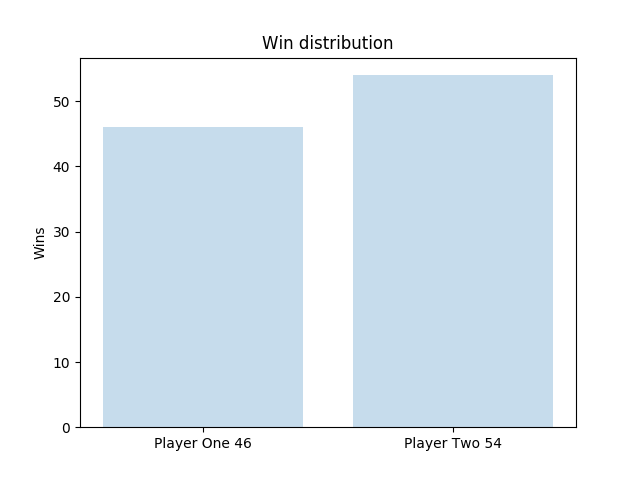
\includegraphics[width=0.66\textwidth]{Results-01}
  \caption{Example results for two player Rochambeau after 100 games.}
  \label{fig:Results-01}
\end{figure}

\mysubsection{2}{b}
When we add a third player that plays a fixed strategy of always choosing paper we get a following distribution of wins after 100 games, see \cref{fig:Results-03}.

\begin{figure}[H]
  \centering
  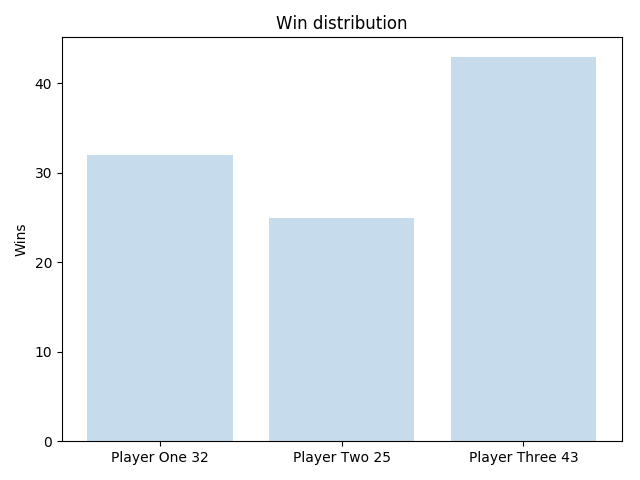
\includegraphics[width=0.5\textwidth]{Results-03}
  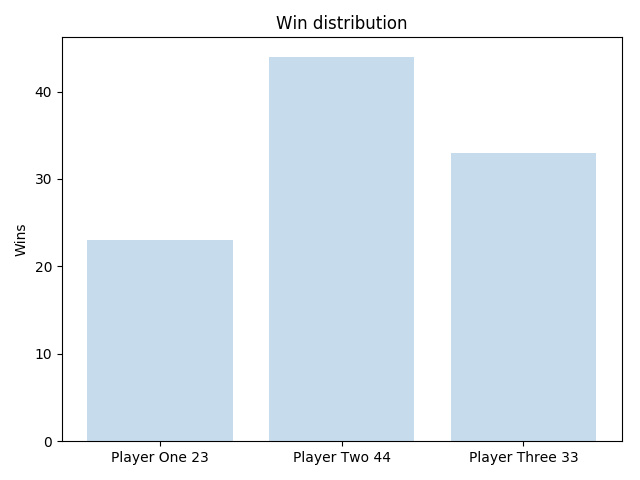
\includegraphics[width=0.5\textwidth]{Results-04}
  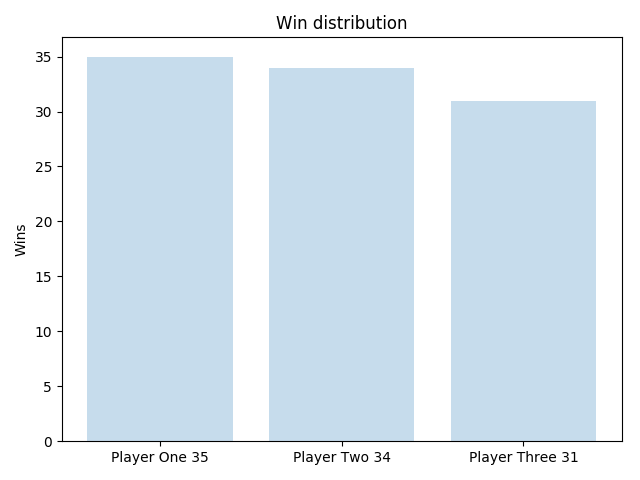
\includegraphics[width=0.5\textwidth]{Results-05}
  \caption{Example results for three player Rochambeau after 100 games.}
  \label{fig:Results-03}
\end{figure}

\mysubsection{3}{c}
This result is to be expected and after an infinite amount of games, no player will have advantage over another player. This is exemplified in \cref{fig:Results-02}

\begin{figure}[H]
  \centering
  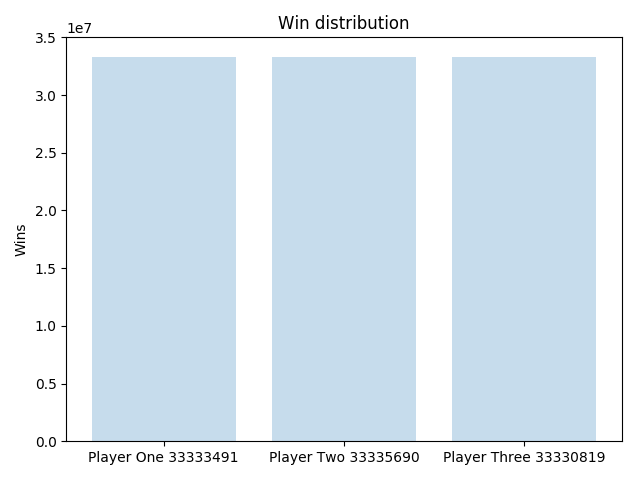
\includegraphics[width=0.66\textwidth]{Results-02}
  \caption{Example results for three player Rochambeau game after 100 million games.}
  \label{fig:Results-02}
\end{figure}

The cause of it is engrained in the way the game is played. Following \cref{tab:outcomes} shows all possible outcomes for each game. As we can clearly see from it, every player has an equal chance of winning. So they will never manage to beat the one that plays a fixed strategy.

\begin{table}[H]
  \centering
  \begin{tabular}{|c|c|c|c|}
    \hline
    \textbf{Player 1} & \textbf{Player 2} & \textbf{Player 3} & \textbf{Outcome} \\ \hline
    Rock              & Rock              & Paper             & Player 3 wins    \\
    Rock              & Paper             & Paper             & Draw             \\
    Rock              & Scissors          & Paper             & Draw             \\
    Paper             & Rock              & Paper             & Draw             \\
    Paper             & Paper             & Paper             & Draw             \\
    Paper             & Scissors          & Paper             & Player 2 wins    \\
    Scissors          & Rock              & Paper             & Draw             \\
    Scissors          & Paper             & Paper             & Player 1 wins    \\
    Scissors          & Scissors          & Paper             & Draw             \\ \hline
  \end{tabular}
  \caption{Table of all possible outcomes when one player plays fixed strategy.}
  \label{tab:outcomes}
\end{table}

Only way for them to beat the player with fixed strategy would be to have some sort of learning algorithm that would let them remember last moves and results of the last matches, increase or decrease a possibility of a certain move based on that and lastly to decay that knowledge to remove an old bias.

\end{document} 